\documentclass[a4paper, 10pt]{article}

\NeedsTeXFormat{LaTeX2e}

%---------------------------- PACKAGE INCLUSION -------------------------------
% This group renders characters clearer and more precise

\RequirePackage[bitstream-charter,cal,expert]{mathdesign}
\RequirePackage{latexsym}

\usepackage{geometry} % to change the page dimensions
\geometry{a4paper,
		  %showframe=true,
		  %margin=3em,
		  %a4paper,
		  %total={170mm,257mm},
		  top=4.15em,
		  left=3em,
		  right=3em,
		  bottom=3.39em
		  }
	
\usepackage{graphicx}  

\usepackage{multicol}  	  

\usepackage{caption}		  
		  		  
\usepackage[default]{cantarell}
\usepackage{xspace}
\usepackage{paralist}
\usepackage[parfill]{parskip} % Activate to begin paragraphs with an empty line rather than an indent
\usepackage{graphicx} % support the \includegraphics command and options
\usepackage{verbatim}
\usepackage{epsfig}
\usepackage{booktabs}

\usepackage{listings}
\usepackage[lined,resetcount]{algorithm2e}
\usepackage{proof}
\usepackage{relsize}
\usepackage{appendix}
\usepackage{tabularx,caption}
		  		  
\newcommand{\EmbedCode}[3]{
	\lstset{language=#1, frame=none, backgroundcolor=\color{white},
			rulecolor=, xleftmargin=5.0ex}
	%\lstset{linewidth=\columnwidth}
	\lstset{commentstyle=\textit, stringstyle=\upshape,showspaces=false}
	\lstset{frame=none, showstringspaces=false, numbers=#3,
			numberblanklines=false}
	\lstinputlisting[]{#2} 
}

\usepackage{amsmath}

\usepackage{xcolor}
\definecolor{yerothColorOrange}{RGB}{242, 161, 0}   
\definecolor{yerothColorBlue}{RGB}{77 , 93 , 254}
\definecolor{yerothColorRed}{RGB}{254, 48 , 48}
\definecolor{yerothColorDarkgray}{RGB}{60, 60 , 60}
\definecolor{yerothColorIndigo}{RGB}{83, 0, 125}
\definecolor{yerothColorGreen}{RGB}{2  , 160, 70}
\definecolor{forestgreen}{RGB}{2,160,70}    
\definecolor{mediumblue}{RGB}{7,43,205}    
\definecolor{firebrickred}{RGB}{178,34,34}
\definecolor{listingray}{gray}{0.9}
\definecolor{lbcolor}{rgb}{0.9,0.9,0.9}
\definecolor{darkgreen}{rgb}{0,0.35,0}
\definecolor{medgreen}{rgb}{0,0.5,0}
\definecolor{lightgreen}{rgb}{0.5,0.7,0.5}
\definecolor{pmcolour}{rgb}{0.5,0.7,0.5}
\definecolor{medgrey}{rgb}{0.6,0.6,0.6}
\definecolor{purplish}{rgb}{0.4,0,0.6}
\definecolor{brightred}{rgb}{1,0.2,0.2}

\newcommand{\diplinfn}{DR.\xspace}

\newcommand{\erpsoftwaresystem}{ERP~software--system\xspace}

\newcommand{\yerothrc}{\textcolor{yerothColorGreen}
			{\textsc{\textcolor{yerothColorRed}{YEROTH}}$_{\text{r\&c}}$\xspace}}

\newcommand{\yerotherpblack}{YEROTH--ERP--$3.0$\xspace}

\newcommand{\yerotherp}{\textsc{\textcolor{yerothColorBlue}{YEROTH--ERP--$3.0$}}\xspace}

\newcommand{\myfullacademicname}{DR. XAVIER NOUMBISSI NOUNDOU\xspace}

\usepackage{hyperref}
\hypersetup{
    colorlinks,
	pagebackref,
    citecolor=medgreen,
    linkcolor=purplish,
    breaklinks,
    pdftex,
    bookmarks,
    plainpages=false,
	pdftitle={Information Brochure of the \erpsoftwaresystem \yerotherpblack by: ''\myfullacademicname''.},
    pdfauthor={DR. XAVIER NOUMBISSI NOUNDOU}
}

\usepackage{url}

\newcommand{\all}{<< CMUP >>\xspace}
\newcommand{\defdeo}{<< DEF\_DEO >>\xspace}
\newcommand{\fifo}{<< FIFO >>\xspace}
\newcommand{\lifo}{<< LIFO >>\xspace}

\newcommand{\administrator}{<< Administrator >>\xspace}
\newcommand{\manager}{<< Business manager >>\xspace}
\newcommand{\seller}{<< Seller >>\xspace}
\newcommand{\inventorystockmanager}{<< Stock manager >>\xspace}
\newcommand{\storekeeper}{<< Storekeeper >>\xspace}
\newcommand{\cashier}{<< Cashier >>\xspace}

\newcommand{\adminb}{\textbf{<< Administrator >>}\xspace}
\newcommand{\managerb}{\textbf{<< Business manager >>}\xspace}
\newcommand{\sellerb}{\textbf{<< Seller >>}\xspace}
\newcommand{\inventorystockmanagerb}{\textbf{<< Stock manager >>}\xspace}
\newcommand{\storekeeperb}{\textbf{<< Storekeeper >>}\xspace}
\newcommand{\cashierb}{\textbf{<< Cashier >>}\xspace}

\newcommand{\company}[1]{\textbf{#1}\xspace}
\newcommand{\diplinf}{\textsc{\diplinfn}}
\newcommand{\mariadb}{\texttt{'MariaDB'}\xspace}

\newcommand{\emphbf}[1]{\emph{\textbf{#1}}\xspace}
\newcommand{\emphit}[1]{\emph{\textit{#1}}\xspace}
\newcommand{\mycheckmark}[1]{\textcolor{#1}{$\checkmark$}\xspace}
\newcommand{\mytimes}[1]{\textcolor{#1}{$\times$}\xspace}
\newcommand{\mytimespartial}[1]{\textcolor{yerothColorBlue}{$\checkmark$~(#1)}\xspace}
\newcommand{\boldsc}[1]{\textbf{\textsc{#1}}\xspace}

\newcommand{\bergmann}{Bergmann Automaten GmbH}
\newcommand{\unibremen}{University of Bremen}

\usepackage[T1]{fontenc}
\newcommand{\changefont}[3]{
\fontfamily{#1} \fontseries{#2} \fontshape{#3} \selectfont}
\changefont{cmss}{m}{n}

% Set font to avant-garde
%\renewcommand*\rmdefault{pag}

\pagenumbering{arabic}

\usepackage{fancyhdr}
\pagestyle{fancy}
\renewcommand{\headrulewidth}{0pt}
\rhead{\textbf{\yerothrc}}
\lhead{Information Brochure of the \erpsoftwaresystem \yerotherpblack}
\lfoot{{\small Author: \myfullacademicname}}
\rfoot{{\small Version of --~December~$27$,~$2020$~--}}
\cfoot{\thepage}

%Remove widows and orphants
\clubpenalty = 10000
\widowpenalty = 10000
\displaywidowpenalty = 10000

\fancypagestyle{OnlyFirstPage}{%
	\lhead{}
	\rhead{}
    \lfoot{}
}

\begin{document}

\thispagestyle{OnlyFirstPage}

{\bf \LARGE \yerothrc} {| \sc \scriptsize information brochure of the \erpsoftwaresystem \yerotherpblack}

\vspace{2.0em}

\begin{center}
{\LARGE Information Brochure of the \\
    \vspace{0.3em}
    \erpsoftwaresystem \\
    \vspace{0.5em}
    \yerotherpblack}
\end{center}

\vspace{2.0em}

\begin{center}
{\large \myfullacademicname}
\end{center}

\vspace{1.0em}

\begin{multicols}{2}

\end{multicols}

\begin{table*}[!htbp]
\centering
\resizebox{\textwidth}{!}{%to fit the table within the text width
\begin{tabular}{lccccc}
\centering 
\textbf{Tasks} 	& \managerb 	& \sellerb				& \inventorystockmanagerb 	& \storekeeperb	&	\cashierb 		\\ \hline
insert stock (or service)		& \mycheckmark{yerothColorGreen}	& \mytimespartial{SERVICES}	& \mytimespartial{MERCHANDISE}	& 	&  				 		\\ \hline
delete stock 					& \mycheckmark{yerothColorGreen}	&		& 						&   &  							\\ \hline
view stock 						& \mycheckmark{yerothColorGreen}	& \mycheckmark{yerothColorGreen} & \mycheckmark{yerothColorGreen} & \mycheckmark{yerothColorGreen}	& \mycheckmark{yerothColorGreen} 	\\ \hline
modify stock 					& \mycheckmark{yerothColorGreen}	&	& \mycheckmark{yerothColorGreen}		& 		&  				 		\\ \hline
transfer stock					& \mycheckmark{yerothColorGreen}	&	& \mycheckmark{yerothColorGreen}		& \mycheckmark{yerothColorGreen}	&  		\\ \hline
modify stock 					&  			& 			& 	& 					&	 								\\ 
management strategy  		& \mycheckmark{yerothColorGreen} 	& \mytimespartial{NOT PERMANENT}	& \mytimespartial{NOT PERMANENT}	& 	&  		\\ 
(e.g.: \fifo, etc.)				&				 		&		&				&						&				\\ \hline
point--of--sale 		& \mycheckmark{yerothColorGreen}	& \mycheckmark{yerothColorGreen}	&						& 	& \mycheckmark{yerothColorGreen} \\ \hline
view stock transfers 		 	& \mycheckmark{yerothColorGreen}	&						& \mycheckmark{yerothColorGreen}	& \mycheckmark{yerothColorGreen}	&  							\\ \hline
supplier management 			& \mycheckmark{yerothColorGreen}	& \mycheckmark{yerothColorGreen}	& 						& 			&  	\\ \hline
customer relationship management (CRM) 	& \mycheckmark{yerothColorGreen}	& \mycheckmark{yerothColorGreen}	& 						& 			&  	\\ \hline
business dashboard 				& \mycheckmark{yerothColorGreen}	& 	&					& 									&  \\ \hline
sale return 					& \mycheckmark{yerothColorGreen}	& 	&					& 									&  \\ \hline
view sales information 			& \mycheckmark{yerothColorGreen}	& \mytimespartial{SELF}	&						& 			& 	\\ 	 				
\end{tabular}}
\caption{\yerotherpblack functions--tasks, and associated users--roles.}
\label{tachesEtFonctions}
\end{table*}

\begin{multicols}{2}

\section{Developer Biography}\label{chap:biography}
\vspace{-0.9em}

\begin{center}

\includegraphics[scale=0.32]{../../francais/images/XavierNOUNDOU-2}
\captionof{figure}{Portrait of PR. XAVIER.\label{fig:xaviernoumbis}}
\end{center}

\textbf{\myfullacademicname} is a CHRISTIAN BY FAITH,
Cameroonian, born on September~$16$ $1983$ in
DOUALA (LITTORAL region, CAMEROON).

Xavier has a \textit{''Diplom--Informatiker (Dipl.--Inf.)''}
qualification from the \textbf{\unibremen, Bremen, Bremen, GERMANY} (May~$25$, $2007$).

Xavier is a \textit{PH.D. in Software Engineering}
(software construction, and testing) since November~$18$,~$2020$
because of his academic research, and professional engineering
contributions as follows:


\begin{enumerate}
%	\itemsep -0.7em
	\item 'Context-Sensitive Staged Static Taint Analysis
			For C using LLVM'
		\begin{enumerate}[1.]
			\itemsep -0.7em
			\item source code: \\
			\url{http://github.com/xnoumbissinoundou/yeroth-saint}
			\item full text (published on July~$1^\text{st}$, $2015$): \url{http://archive.org/details/saint_201507}.
		\end{enumerate}		 

	\item 'YEROTH-ERP-3.0':
			\begin{enumerate}[1.]
			\itemsep -0.7em
			\item source code: \\
			\url{http://github.com/xnoumbissinoundou/yeroth-erp-3.0}
			\item full text (ongoing publication): \url{http://archive.org/details/yeroth-erp-3-0-info-english}.
		\end{enumerate}	
\end{enumerate}


\vspace{-1em}

\section{Introduction}

\yerotherpblack is an \textbf{Enterprise Resource Planing} (ERP)
software--system. 

Users of \yerotherpblack could have the following roles:
\begin{enumerate}
	\itemsep -0.4em
	\item \administrator
	\item \manager
	\item \cashier
	\item \seller
	\item \inventorystockmanager
	\item \storekeeper.
\end{enumerate}

\yerotherpblack allows for business management tasks 
listed in Table~\ref{tachesEtFonctions},
depending on user role.

\section{Advantages of \yerotherpblack}

\begin{enumerate}
	\itemsep 0em
	\item \yerotherpblack is $100\%$ stable

	\item \yerotherpblack has an alert system with two types of alerts:
	      alerts based on stock--quantity, and time--period alerts

	\item users have the choice between small size receipts,
	      and, bigger size receipts (''A4'')

	\item \yerotherpblack runs on the Linux operating system,
	      because Linux is stable, performant, and less
	      vulnerable to security breaches in comparison
	      to other operating systems ('\texttt{Windows~$10$}')

	\item \yerotherpblack has an user interface ''Sales'' to view
		  sale information~(Figure~\ref{fig:fenetre-de-la-vente}),
		  and thus enables users to make managerial decisions

	\item \yerotherpblack has an interface ''Business dashboard'' that
		  generates financial accounting reports,
		  from sale and payment information, to help
		  managers to make ''business decisions''.
\end{enumerate}

\vspace{1em}

\begin{center}
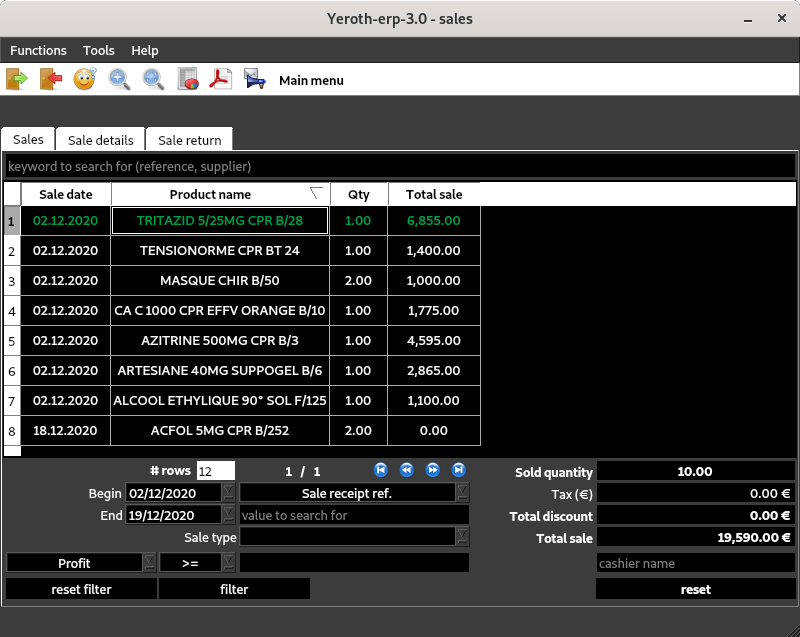
\includegraphics[scale=0.32]{images/yeroth-erp-3-0-sale-information.png}
\captionof{figure}{Sale--information window.\label{fig:fenetre-de-la-vente}}
\label{fig:fenetre-de-la-vente}
\end{center}

\vspace{0.1em}

\section{Alert System}
\vspace{-0.3em}
Users with roles \administrator or \manager
are the ones able to create alerts.

\yerotherpblack allows its users to create two
types of alerts:
\begin{enumerate}
  \itemsep -0.5em
  \item alerts over stocks--quantities
  \item alerts over time intervals (this helps for
	  perissable articles and for sales discounts
	  over a period of time).
\end{enumerate}

\subsection{Alerts over Stock--Quantity}

An alert aver a stock--quantity is a message that
is sent to a pre--determined user whenever
''pre--determined'' stock--quantity (X) of
a specific article--stock is reached.

For instance, Xavier (\manager) could create
an alert for stock ''mango'' that will be
trigerred whenever stock ''mango'' quantity
reaches $100$; An alert--message is sent
to user John (\storekeeper).

\subsection{Alerts over Time--Period}

A time--period is defined by a
starting--date and an ending--date
(dates are from the ''gregorian'' calendar).

An alert aver a time--period (T) is a message
that is generated, sent to a pre--determined user,
and kept within \yerotherpblack from T's starting--date 
up to T's ending--date.

For example, an alert with a message has to be
sent to Paul (\cashier) when the date of May
$05^{th}$ is reached. The alert message
specifies that a rebate of $20\%$ has to be applied
on every sale of yoghourt 'tr\`esbon' during a
time interval of $2$ weeks.

\vspace{-1.0em}

\section{Database Management System}
\vspace{-0.3em}
\yerotherpblack uses \mariadb as the standard DBMS. 
\mariadb is very stable, very performant,
and free--software.

\vspace{-0.7em}

\section{Conclusion}
\begin{center}
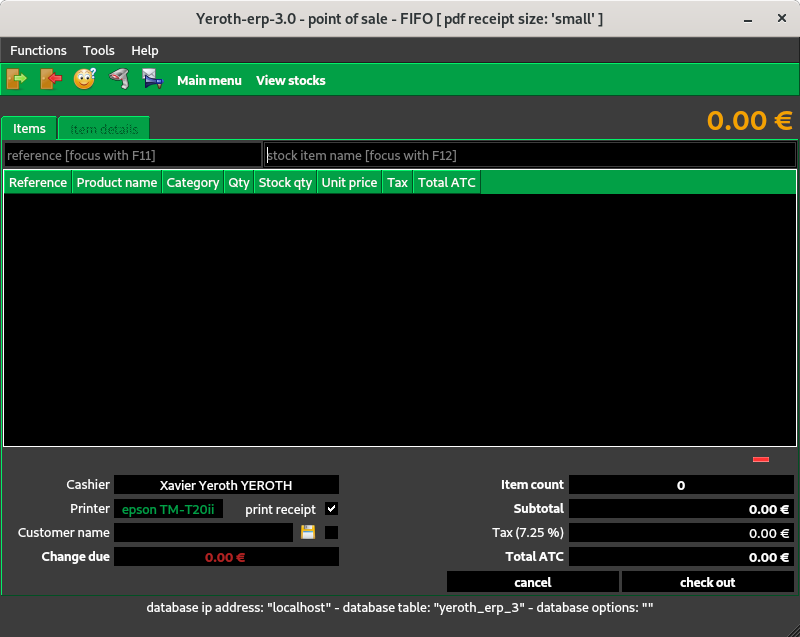
\includegraphics[scale=0.33]{images/yeroth-erp-3-0-window-cashier.png}
\captionof{figure}{Point--of--sale window.}
\label{fig:fenetre-de-vente}
\end{center}

Figure~\ref{fig:fenetre-de-vente} illustrates
the window for selling articles.

\begin{center}
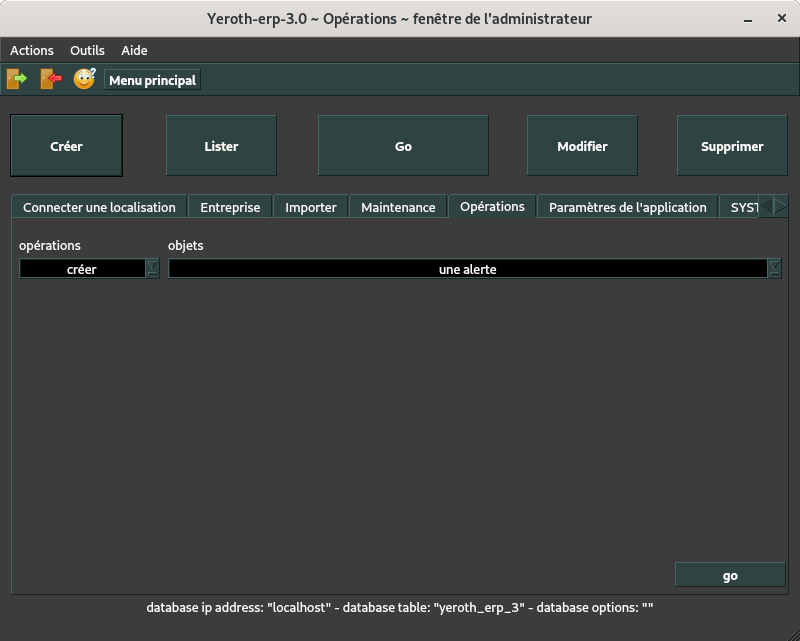
\includegraphics[scale=0.33]{images/yeroth-erp-3-0-admin-view-window.png}
\captionof{figure}{Administrative window for business manager.}
\label{fig:fenetre-de-stock}
\end{center}

Figure~\ref{fig:fenetre-de-stock} illustrates
the administrative window for business managers.

\end{multicols}

\end{document}
